\clearpage
\section{Recordatorios asociados a localizaciones} \label{sec:recordatorios}

En esta última práctica se propone crear una aplicación que permita al usuario gestionar una serie de recordatorios, pero en vez de estar asociados estos recordatorios a un instante de tiempo en concreto, se asocien a un área geográfica concreta. Vamos a definir esta área como una circunferencia de 100 metros de radio alrededor de un punto geográfico que será definido por el usuario cuando cree el recordatorio. A esta circunferencia la llamaremos ``área de influencia''. Para ello, el usuario seleccionara un punto sobre el mapa y asignará un nombre y una descripción para este recordatorio.

\begin{figure}[H]
\centering
    \centering
        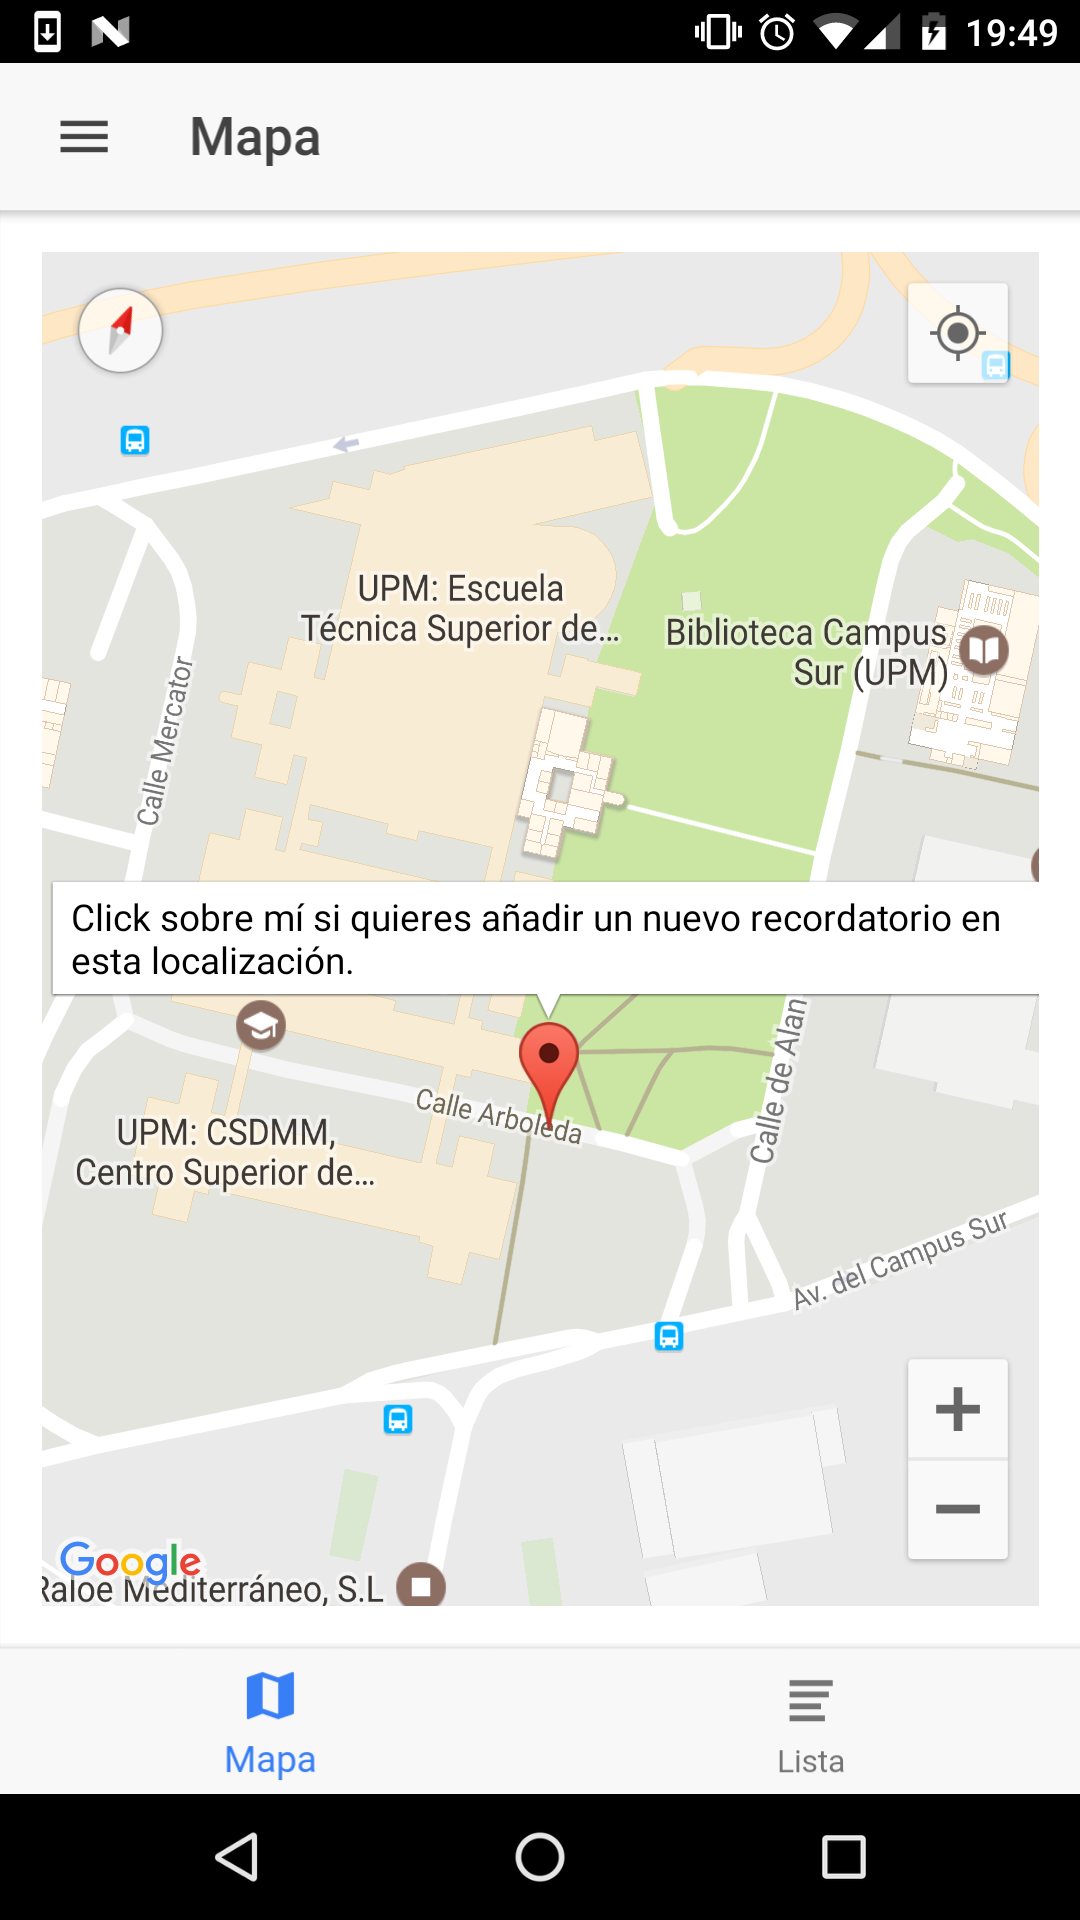
\includegraphics[width=0.4\textwidth]{Figures/ch2/ReminderMap/preview_map_1}
        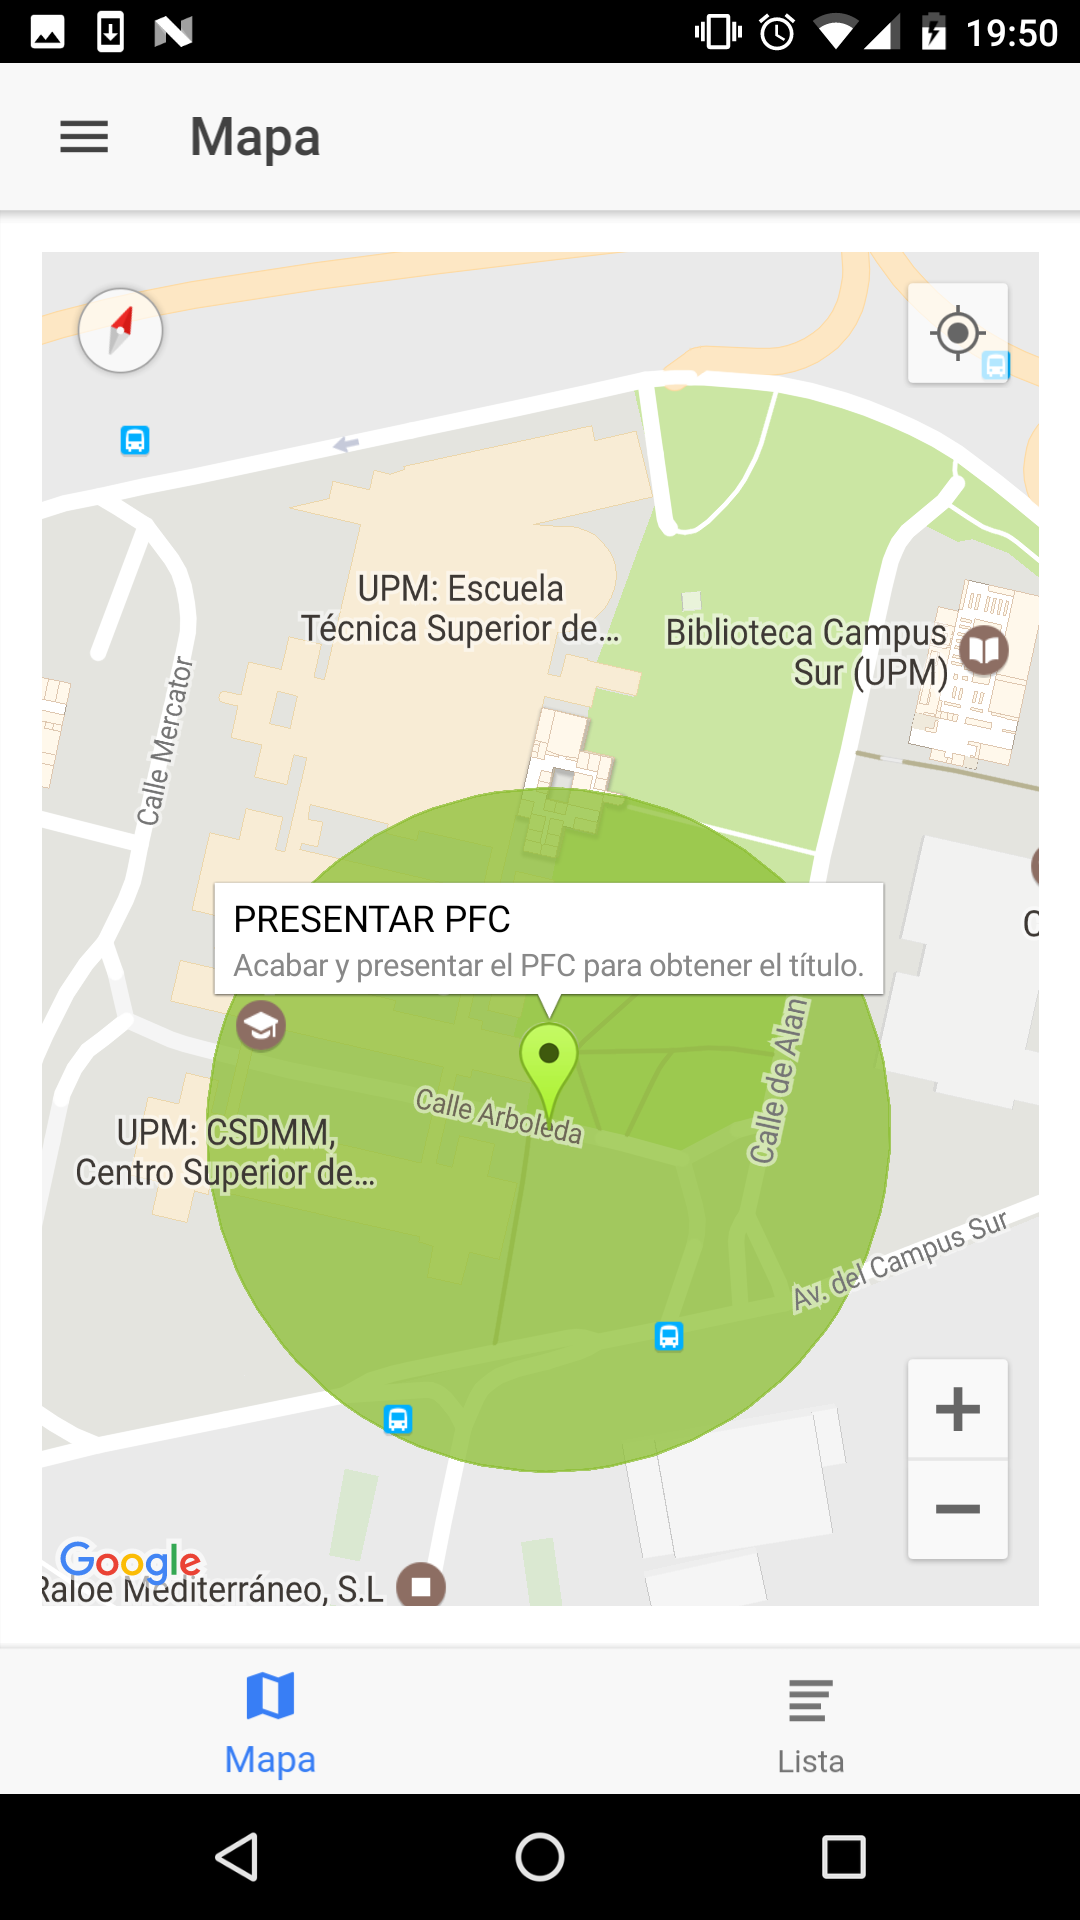
\includegraphics[width=0.4\textwidth]{Figures/ch2/ReminderMap/preview_map_2}
    \caption{Así se vería el mapa, con los recordatorios marcados.}
\end{figure}

También podremos ver estos recordatorios listados, pudiendo interactuar con ellos:

\begin{figure}[H]
\centering
    \centering
        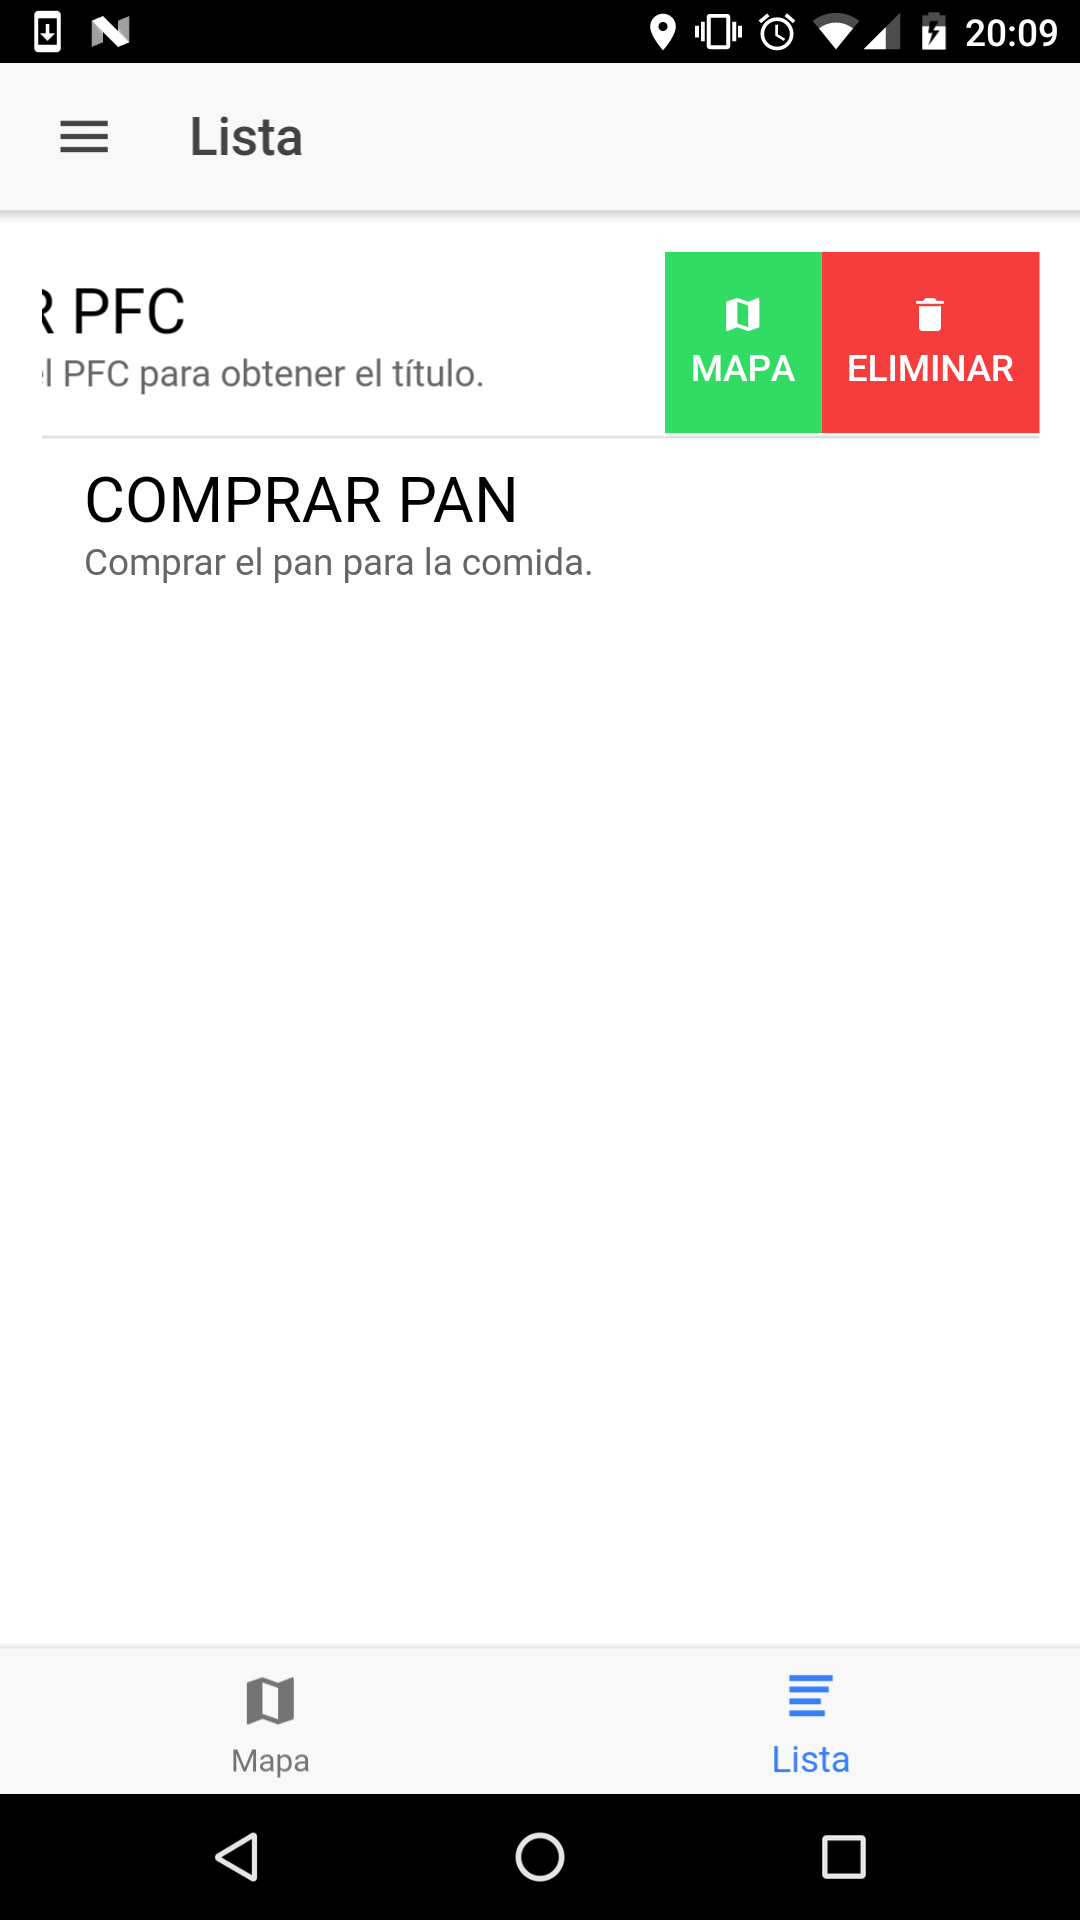
\includegraphics[width=0.4\textwidth]{Figures/ch2/ReminderMap/preview_list}
    \caption{Aquí vemos la lista de recordatorios, sobre los que podremos interactuar.}
\end{figure}

Los recordatorios quedarán almacenados de manera persistente en la \gls{BBDD} que implementa el sistema operativo, así, la información no se perderá al cerrar la aplicación ni al apagar el dispositivo.

Y como objetivo último de la aplicación, se notificará al usuario de que cerca de la zona en la que se encuentra, tiene registrado un recordatorio. Dicha notificación  se activará al entrar dentro del área de influencia de este:

\begin{figure}[H]
\centering
    \centering
        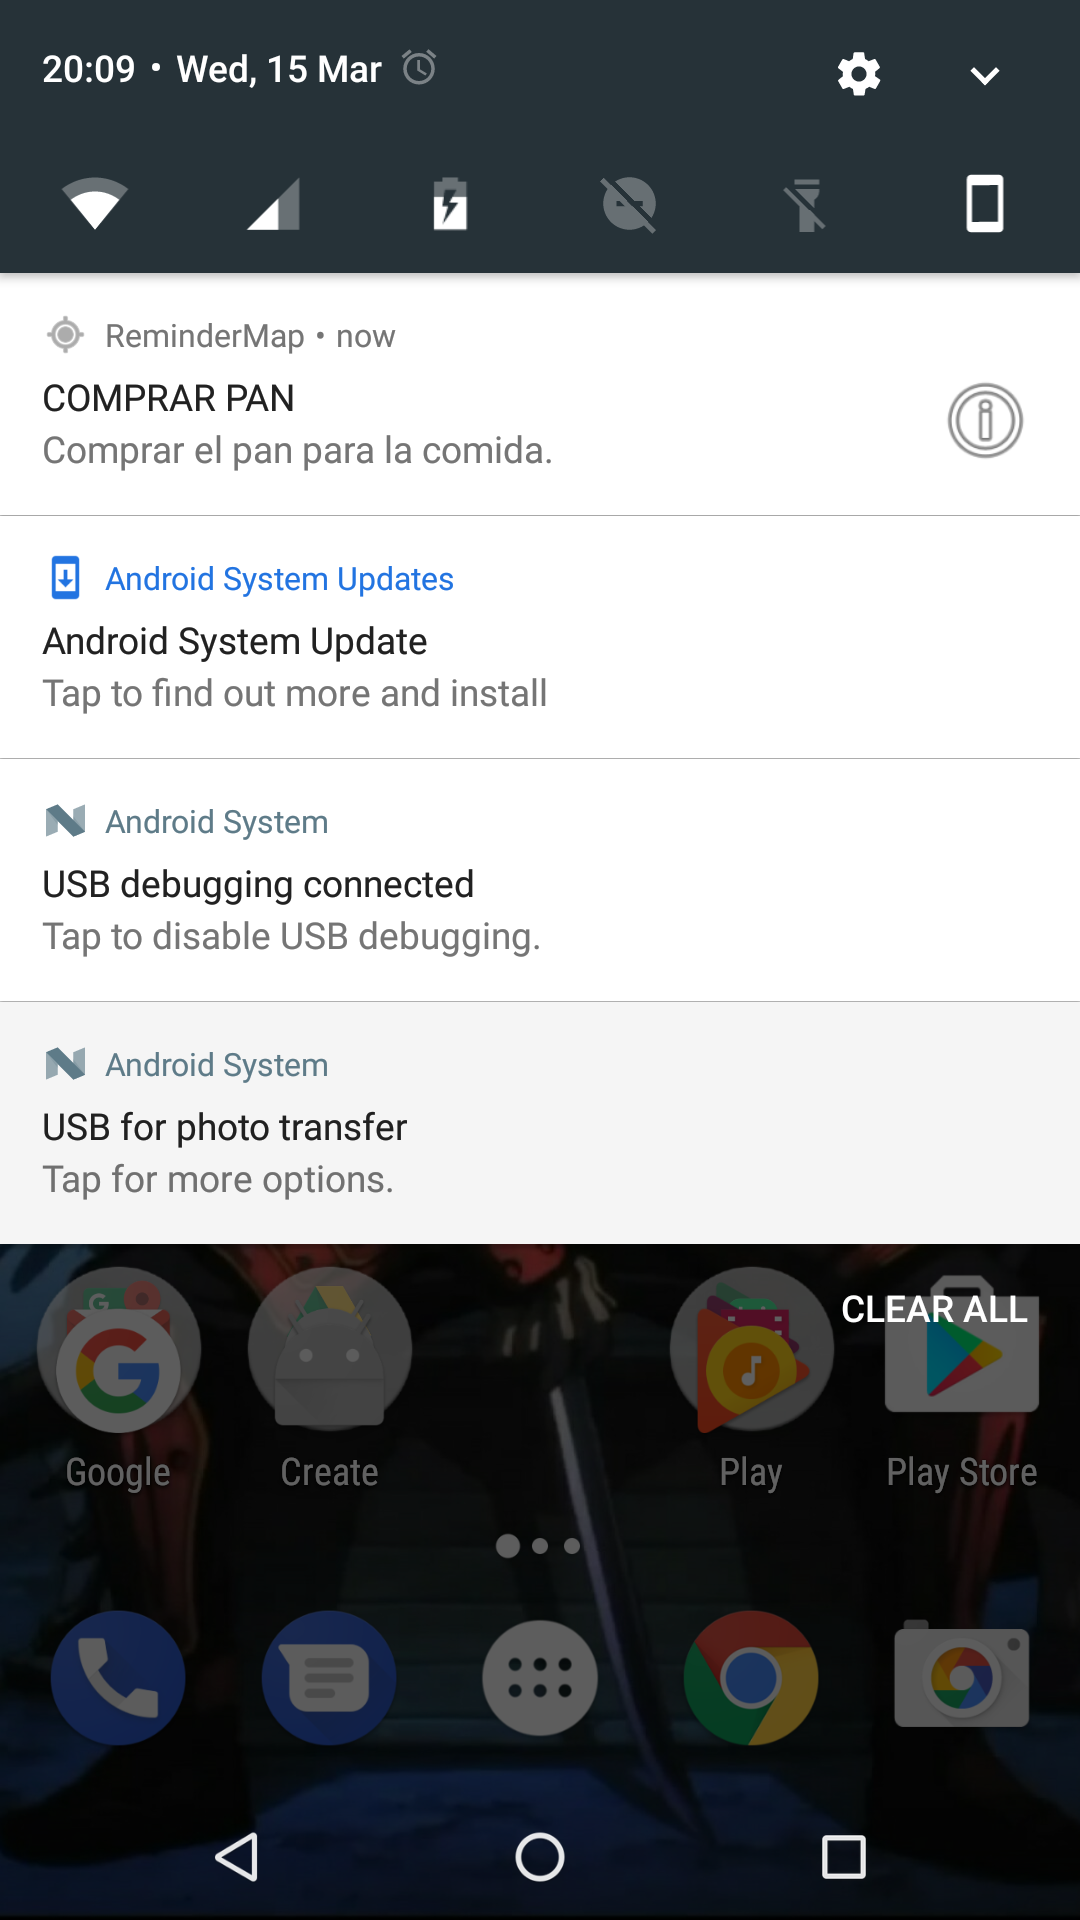
\includegraphics[width=0.4\textwidth]{Figures/ch2/ReminderMap/preview_alert}
    \caption{La notificación aparece aunque no este abierta la aplicación.}
\end{figure}

Para el desarrollo de esta aplicación se vamos a usar algunos módulos de Ionic Native. Como ya se vio en el apartado dedicado a \nameref{subsec:IonicNative}, se trata de un conjunto de envoltorios sobre algunos de los plugins con los que cuenta Cordova facilitando así su uso desde nuestro código escrito en TypeScript.

Entre todos los plugins disponibles, vamos a usar los siguientes:

\begin{enumerate}
  \item Google Maps\footnote{\url{https://ionicframework.com/docs/native/google\-maps/}}: Nos permitirá manejar de manera sencilla datos geográficos y visualizarlo sobre un mapa, crear y manipular estos mapas, acceder a los datos de geolocalización del dispositivo, \ldots para ello utiliza el SDK nativo de Google Maps.
  \item GeoFence\footnote{\url{https://ionicframework.com/docs/native/geofence/}}: También relacionado con la localización, pero implementado en un plugin diferente al anterior, nos permite crear alertas para cuando el dispositivo entre dentro de una zona geográfica definida. Estas alertas se mantienen incluso con la aplicación apagada.
  \item SQLite\footnote{\url{https://ionicframework.com/docs/native/sqlite/}}: Nos permite acceder a la \gls{BBDD} del dispositivo pudiendo hacer que nuestros datos sean persistentes mediante consultas \gls{SQL}
\end{enumerate}

Además, vamos a aprovechar esta práctica para ver como hacer uso de dos componentes de Ionic2 que son los \emph{tabs o pestañas} y el \emph{sidemenu o menú lateral}. Ambos componentes son muy utilizados en aplicaciones de todo tipo donde se quiere facilitar al usuario la navegación entre las diferentes páginas que la componen.

\subsubsection{Análisis funcional}

En esta aplicación se van a usar varios elementos como varias páginas, servicios, modelos de datos, plugins de Cordova, \ldot por lo que es interesante realizar un análisis funcional para tener una visión de los elementos que compondrán la aplicación y como interactúan entre ellos.

\begin{figure}[H]
\centering
    \centering
        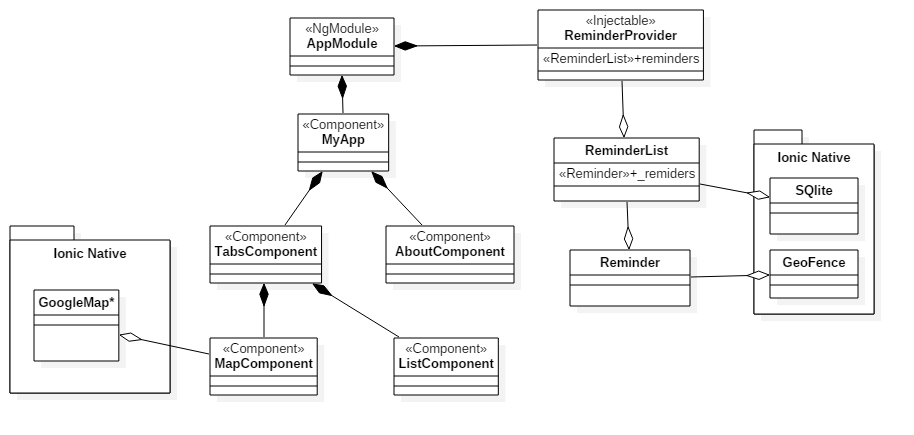
\includegraphics[width=0.8\textwidth]{Figures/ch2/ReminderMap/class_diagram}
    \caption{Diagrama de clases.}
\end{figure}

En el diagrama podemos ver como de nuestro módulo único parten las diferentes páginas de la aplicación. En primer lugar encontramos la página \emph{MyApp}, de la cual cuelgan todas las demás. \emph{MyApp} contendrá el menú lateral y desde el que se accederá a las páginas \emph{TabsComponent} y \emph{AboutComponent}. A su vez, \emph{TabsComponent} actuará de contenedor para \emph{MapComponent} y \emph{ListComponent}.

Por otro lado tenemos la clase \emph{Reminder}, que actuará como modelo y representará un recordatorio. Por encima de esta clase, se encuentra \emph{ReminderList}, que actuara como \emph{manager}, facilitando el manejo de los recordatorios y de la comunicación con la \gls{BBDD}.

También existirá un \emph{provider} que se usará para compartir inicializar un \emph{ReminderList} y que pueda ser compartido por todos los componentes de nuestra aplicación que lo necesiten, en nuestro caso, los componentes \emph{MapComponent} y \emph{ListComponent}. Esto se consigue utilizando el \emph{Dependency Injector} de Angular (ver \ref{sec:angular}).

Por último podemos ver el uso de los plugins de Ionic Native, comentados en la introducción, por parte de algunas de las clases.

\subsubsection{Estructura de las páginas}

En primer lugar vamos a crear las paginas de la aplicación y la navegación entre ellas. El aspecto que queremos tener en nuestra aplicación, y la navegación entre páginas se puede ver de manera gráfica en el siguiente esquema.

\begin{figure}[H]
\centering
    \centering
        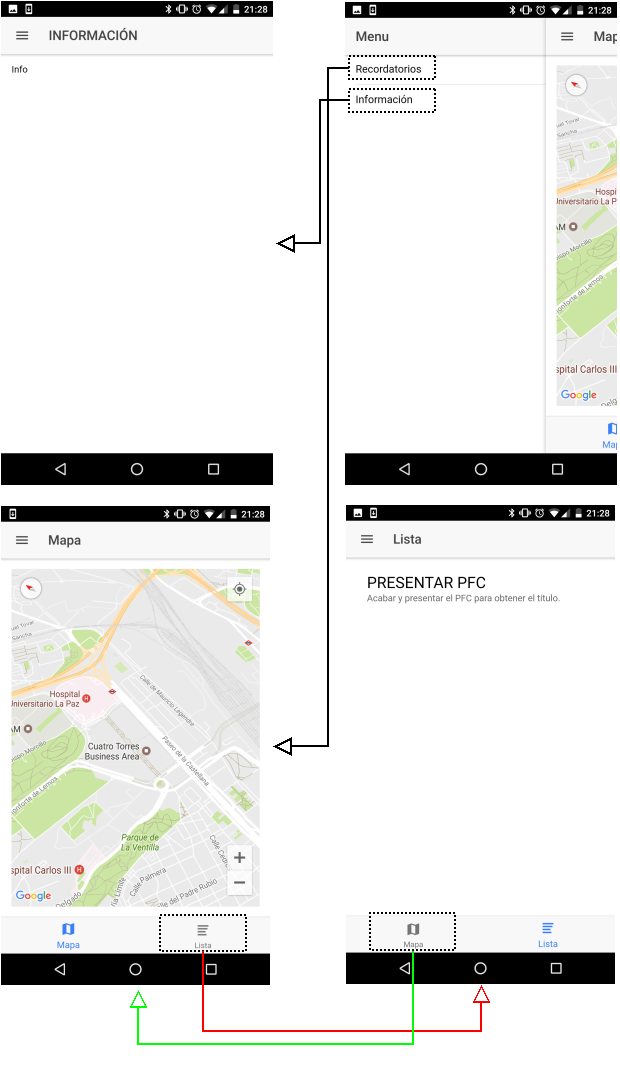
\includegraphics[height=0.7\textheight]{Figures/ch2/ReminderMap/mockup}
    \caption{Mockup de la aplicación. Podemos ver los enlaces entre páginas y los menús desde las que se acceden.}
\end{figure}

Necesitaremos implementar cuatro páginas diferentes para nuestra aplicación:

\begin{enumerate}
  \item Un una de las páginas se colocarán la barra de \emph{tabs} en la parte inferior. Además, deberá servir de contenedor para las siguientes dos páginas.
  \item Una página mostrará el mapa y que irá contenida en la anterior.
  \item Similar a la anterior, necesitaremos otra página para mostrar la información pero en formato de lista y también contenida en la primera.
  \item Una última página, esta vez dependiente de la página de \emph{tabs}, para mostrar la información sobre la aplicación.
\end{enumerate}

A su vez, como ocurre en todos los proyectos, estas páginas estarán contenidas dentro del componente padre de la aplicación, \emph{app}, y que será donde se implementará el menú lateral.

Vamos a empezar, pero en esta ocasión, en vez de usar un \emph{starter} vacío como era \emph{blank}, vamos a utilizar uno que ya implementa un menú lateral y al que iremos añadiendo nuestra páginas. Este \emph{starter} lo podemos encontrar en el market de Ionic2 y nos va a proporcionar la base para empezar una aplicación que cuente con un menú lateral. He aquí la importancia de revisar este market antes de ponerse a desarrollar por si podemos aprovechar lo ya desarrollado por otra persona.

Iniciamos nuestro proyecto con el siguiente comando, en el que podemos ver que el nombre del \emph{starter} a utilizar es \textbf{sidemenu}:

\begin{lstlisting}[language=bash]
  # ionic start ReminderMap sidemenu --v2
\end{lstlisting}

Si ejecutamos el proyecto tal cual, veremos que podemos abrir un menú lateral en el que aparecen dos páginas, a las que podemos acceder pulsando sobre ellas.

\begin{figure}[H]
\centering
    \centering
        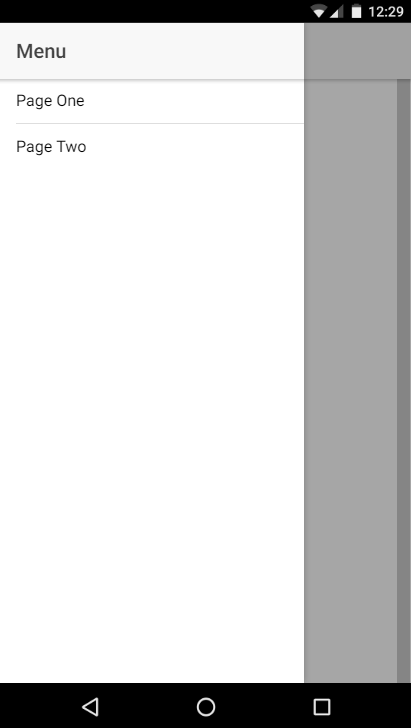
\includegraphics[width=0.4\textwidth]{Figures/ch2/ReminderMap/sidemenu_starter_serve}
    \caption{Menú lateral que nos proporciona la plantilla sidemenu.}
\end{figure}

Estas páginas que vemos se crean por defecto. Pueden ser editadas y añadir así nuestro contenido o, como vamos a hacer nosotros, podemos eliminarlas y crear las nuestras desde cero. Generaremos nuestras páginas utilizando Ionic CLI, consiguiendo que nuestras páginas tengan la estructura necesaria de ficheros usando un único comando. Las páginas a crear son las comentadas unos párrafos atrás:

\begin{lstlisting}[language=bash]
  # ionic generate page tabs
  # ionic generate page map
  # ionic generate page list
  # ionic generate page about
\end{lstlisting}

Empezaremos modificando el menú lateral para que muestre la páginas \emph{tabs} y \emph{about}. A continuación, añadiremos el componente de Ionic \textbf{ion-tabs} a la página \emph{tabs} y enlazaremos las páginas \emph{maps} y \emph{list} a este componente.

Editamos el archivo \emph{/app/app.html}, que actúa como página padre de la aplicación. Aquí vemos la primera implementación que añade el \emph{starter} \textbf{sidemenu}.

\begin{lstlisting}[style=htmlcssjs,frame=tlrb,xleftmargin={0.2cm}]
  <ion-menu [content]="content" >
    <ion-header>
      <ion-toolbar>
        <ion-title>Menu</ion-title>
      </ion-toolbar>
    </ion-header>

    <ion-content>
      <ion-list>
        <button menuClose ion-item *ngFor="let p of pages" (click)="openPage(p)" >
          {{p.title}}
        </button>
      </ion-list>
    </ion-content>

  </ion-menu>

  <!-- Disable swipe-to-go-back because it's poor UX to combine STGB with side menus -->
  <ion-nav [root]="rootPage" #content swipeBackEnabled="false" ></ion-nav>
\end{lstlisting}

Encontramos el componente \textbf{ion-menu}, el cual se inicia con los valores que encuentra dentro de la propiedad \emph{pages}, que pertenece al componente \emph{MyApp} que se encuentra dentro del fichero \emph{app.component.ts}. Lo abrimos y vemos que se trata de un diccionario en el que se indica el título del botón y la página a la que hace referencia. También vemos la función \textbf{openPage}, que es llamada desde los botones del menú (función asignada al evento \emph{click}) y que se encarga de abrir la página correspondiente. Cambiamos pues este diccionario para introducir nuestras páginas de la siguiente forma:

\begin{lstlisting}[style=htmlcssjs,frame=tlrb,xleftmargin={0.2cm}]
    this.pages = [
      { title: 'Recordatorios', component: TabsPage },
      { title: 'Información', component: AboutPage }
    ];
\end{lstlisting}

También cambiamos la variable \textbf{rootPage}, que define la página de inicio, por \textbf{TabsPage}. No nos debemos olvidar de importar nuestras páginas.

Como estamos usando páginas creadas por nosotros, tendremos que declararlas y añadirlas como \emph{entryComponents} \footnote{\url{https://angular.io/docs/ts/latest/cookbook/ngmodule-faq.html}}. Estos cambios se han de realizar en la definición del \emph{ngModule}, en el fichero \emph{app.module.ts}. Eliminamos las páginas que venían definidas en el \emph{starter} y añadimos nuestras  propias páginas.

\begin{lstlisting}[style=htmlcssjs,frame=tlrb,xleftmargin={0.2cm}]
  declarations: [
      MyApp,
      AboutPage,
      TabsPage,
      MapPage,
      ListPage
    ],
    ...
    entryComponents: [
      MyApp,
      AboutPage,
      TabsPage,
      MapPage,
      ListPage
    ]
\end{lstlisting}

Ya tenemos creado nuestro menú lateral con el que acceder a nuestra página principal y a la de información. Ahora vamos a añadir el componente \textbf{ion-tabs} a nuestra página \emph{tabs.html}. La editamos con el siguiente código:

\begin{lstlisting}[style=htmlcssjs,frame=tlrb,xleftmargin={0.2cm}]
  <ion-tabs selectedIndex="0" >
    <ion-tab [root]="mapTabRoot" tabTitle="Mapa" tabIcon="map" ></ion-tab>
    <ion-tab [root]="listTabRoot" tabTitle="Lista" tabIcon="list" ></ion-tab>
  </ion-tabs>
\end{lstlisting}

Como se observa, se han añadido dos \emph{tabs} a los que se les ha definido un texto (atributo \textbf{tabTitle}) y un icono (de los disponibles en la fuente Ionicons y definido por el atributo \textbf{tabTitle}). Con el atributo \textbf{[root]} se indica la página que se debe mostrar al seleccionar esa pestaña. El parámetro que se indica en este atributo debe estar definido como propiedad en el componente de la página, en \emph{TabComponent}:

\begin{lstlisting}[style=htmlcssjs,frame=tlrb,xleftmargin={0.2cm}]
  @Component({
    templateUrl: 'tabs.html'
  })
  export class TabsPage {
    mapTabRoot: any = MapPage;
    listTabRoot: any = ListPage;

    constructor() {}
  }
\end{lstlisting}

Por último, y para acabar con la estructura de páginas que tendrá la aplicación, añadiremos cabeceras que contengan a cada una de las páginas con un título que las identifique junto a un botón con el que abrir el menú lateral. La cabecera para todas ellas sería así:

\begin{lstlisting}[style=htmlcssjs,frame=tlrb,xleftmargin={0.2cm}]
  <ion-header>
    <ion-navbar>
      <button ion-button menuToggle>
        <ion-icon name="menu" ></ion-icon>
      </button>
      <ion-title>INFORMACIÓN</ion-title>
    </ion-navbar>
  </ion-header>
\end{lstlisting}

Esta cabecera deberá ir en todas las páginas menos en la pagina \emph{tabs}, ya que está actúa de contenedor de páginas que poseen su propia cabecera.

\subsubsection{Instalando los plugins necesarios}

Antes de empezar a implementar la lógica, vamos a instalar los plugins que hemos enumerado y que necesitaremos para nuestra aplicación. Los plugins se pueden instalar utilizando Ionic CLI. Se recomienda añadir en primer lugar las plataformas objetivo al proyecto, y a continuación, instalar los plugins. Empecemos:

\begin{lstlisting}[language=bash]
  # ionic platform add android
\end{lstlisting}

Seguimos con un plugin usado para gestionar la política de acceso a páginas desde la aplicación. No lo usaremos directamente, pero es necesario para que nuestro mapa funcione.

\begin{lstlisting}[language=bash]
  # ionic plugin add cordova-plugin-whitelist
\end{lstlisting}

El caso del plugin de Google Maps tiene la particularidad de que hay que indicar que API KEY del servicio debe utilizar ya en el momento de la instalación del módulo. En el anexo \nameref{ch:google_api} podemos ver como conseguir esta API KEY. En el momento de escribir este documento, el plugin se encuentra en la versión 1.4, aunque la versión 2 ya está desarrollada y en fase beta. Vamos a usar la versión 1.4, la cual indicaremos en el comando para asegurarnos de que es la que se instala.

\begin{lstlisting}[language=bash]
  # ionic plugin add cordova-plugin-googlemaps@1.4 --variable API_KEY_FOR_ANDROID=MY_API_KEY
\end{lstlisting}

El resto de plugin no tienen ninguna peculiaridad a destacar.

\begin{lstlisting}[language=bash]
  # ionic plugin add cordova-sqlite-storage
  # ionic plugin add cordova-plugin-geofence
\end{lstlisting}

Cabe destacar la facilidad que ofrece no Ionic a la hora de añadir nuevos plugin a cualquier aplicación.

\subsubsection{Implementación del modelo de datos y la persistencia}

Como hemos visto en el análisis, nuestra aplicación va a contar con una clase que actúe de modelo y que contenga la información de un recordatorio. Ya que la aplicación podrá manejar varios recordatorios, y estos deberán ser guardados en la \gls{BBDD} del dispositivos y poder ser recuperados de ella, se implementará una clase que abstraiga de estas tareas al resto de clases.

\tipbox{Como ocurre en muchos otros lenguajes, existen módulos para Ionic2 que implementan el modelo \gls{ORM}\footnote{\url{https://github.com/BradyLiles/ionic-orm}}. Este modelo se basa en el mapeado de las tablas de una \gls{BBDD} en entidades que simplifiquen las tareas básicas de acceso a esas tablas.}

Vamos a empezar definiendo la clase \emph{Reminder} que actuara de modelo para nuestros recordatorio.

\begin{lstlisting}[style=htmlcssjs,frame=tlrb,xleftmargin={0.2cm}]
  export class Reminder {
    private _id: number;
    private _name: string;
    private _description: string;
    private _lat: number;
    private _lng: number;

    constructor(name: string, description: string,
    latLng: GoogleMapsLatLng | Array<number>, id: number=null) {
      this._id = id;
      this.name = name;
      this.description = description;
      if (latLng instanceof Array) {
        this._lat = latLng[0];
        this._lng = latLng[1];
      } else {
        this._lat = latLng['lat'];
        this._lng = latLng['lng'];
      }
    }

    get id(): number { return this._id;
    }

    get name(): string { return this._name;
    }

    set name(name: string) { this._name = name.substr(0, 16);
    }

    get description(): string { return this._description;
    }

    set description(description: string) {
      this._description = description.substr(0, 512);
    }

    get latLng(): GoogleMapsLatLng {
      return new GoogleMapsLatLng(this._lat, this._lng);
    }

    set latLng(latLng: GoogleMapsLatLng ) {
      this._lat = latLng['lat'];
      this._lng = latLng['lng'];
    }
  }
\end{lstlisting}

Se puede observar que se han declarado las variables privadas y se ha decidido implementar sus métodos \emph{getter} y \emph{setter}. Con esto se consigue tener control sobre asignación de valores a estas variables, como por ejemplo, la longitud del nombre o la imposibilidad de modificar el id. Por otro lado, la localización se define como dos variables, una para la latitud y otra para la longitud, pero a la hora de querer modificar o recuperar esta localización, se usa un objeto de tipo \emph{GoogleMapsLatLng}. Se ha decido hacer esto así ya que este tipo de objetos es el que usa el plugin de Google Map para representar una coordenada geográfica. Pero, ¿y por qué no definirlo también así en nuestro modelo?. La razón es que nuestro modelo va a ser almacenado dentro de una \gls{BBDD}, y no podremos guardar directamente en ella el objeto \emph{GoogleMapsLatLng} directamente, sino que necesitaremos serializarlo o descomponerlo en elementos de tipo básico. Además, no siempre se puede usar \emph{GoogleMapsLatLng} para definir una coordenada, como ya veremos a la hora de usar \emph{GeoFence}.

Implementamos también nuestro \emph{ReminderList}, que tendrá como variable un \emph{Array} de elementos de tipo \emph{Reminder}, el cuál será privado y accedido a través de la función \emph{all()}:

\begin{lstlisting}[style=htmlcssjs,frame=tlrb,xleftmargin={0.2cm}]
  export class ReminderList {
    private _reminders: Array<Reminder>;

    constructor(public events: Events) {}

    all(): Array<Reminder> { return this._reminders;
    }
  }
\end{lstlisting}

Con estas dos clases ya definidas, vamos a ir añadiéndoles funcionalidades. Para empezar, añadiremos persistencia a los datos, es decir, crearemos los métodos necesarios para poder leer y escribir en la \gls{BBDD} del dispositivo. Tendremos que importar la clase \textbf{SQLite} desde el paquete \textbf{ionic-native}.

Para utilizar una \gls{BBDD}, debemos instanciar un objeto de esta clase con el cual podremos abrir una \gls{BBDD} usando el método \textbf{openDatabase} y ejecutar queries sobre ella con el método \textbf{executeSql}. Ambos métodos nos devolverán promesas, en las cuales indicaremos la acción a realizar en función de si la operación haya ido bien o mal. Empecemos viendo como quedaría el constructor de nuestra clase \emph{ReminderList}.

\begin{lstlisting}[style=htmlcssjs,frame=tlrb,xleftmargin={0.2cm}]
  export class ReminderList {
    private _db: SQLite;
    // RESTO DE VARIABLES

    constructor(public events: Events) {
      this._db = new SQLite();
      this._db.openDatabase({
        name: 'reminder.db',
        location: 'default'
      }).then(() => {
        this._db.executeSql('CREATE TABLE IF NOT EXISTS reminders (id INTEGER PRIMARY KEY,' +
          'name VARCHAR(16), description VARCHAR(512), lat FLOAT, lng FLOAT)', []
        ).then((data) => {
            this.refresh();
        }, (err) => {
          console.error('Unable to execute sql: ', err);
        });
      }, (err) => {
        console.error('Unable to open database: ', err);
      });
    }
    // RESTO DE MÉTODOS
  }
\end{lstlisting}

En primer lugar se instancia un objeto \emph{SQLite} el cual asignamos a una propiedad privada de \emph{ReminderList}. Abrimos la \gls{BBDD} con el ya mencionado método \textbf{openDatabase}, al cual se le indica el nombre de la \gls{BBDD} y la localización (usaremos \emph{default}). Si la \gls{BBDD} se ha abierto sin problemas, podremos ejecutar nuestra primera query. Con esta primera query crearemos la tabla en la que se escribirá la información de los recordatorios, solo si no existe ya. Se han definido las columnas acorde al tipo de dato que van a almacenar, además, se ha definido la columna \emph{id} como \textbf{PRIMARY KEY}. Si todo ha ido según se espera, podremos llamar al método \emph{refresh()}, el cual poblará el \textbf{Array} \emph{\_reminder} con la información de la tabla. La definición de este método es la siguiente:

\begin{lstlisting}[style=htmlcssjs,frame=tlrb,xleftmargin={0.2cm}]
  onUpdate: EventEmitter<Array<Reminder>> = new EventEmitter();

  refresh() {
    this._reminders = [];
    this._db.executeSql('SELECT * FROM reminders', []).then(
      (data) => {
          for (let i = 0; i < data.rows.length; i++) {
            let item = data.rows.item(i);
            this._reminders.push(new Reminder(item.name, item.description,
              [item.lat, item.lng], item.id))
          }
          this.onUpdate.emit(this._reminders);
      }, (err) => {
        console.error('Unable to execute sql: ', err);
      }
    )
  }
\end{lstlisting}

En este método se asigna un array vacío a la variable \emph{\_reminder}. Acto seguido, se ejecuta una query \gls{SQL} para recuperar toda la información de la tabla. Si todo ha ido bien, las filas que devuelve la query son mapeados en un \gls{JSON} que se pasa como parámetro a la primera función que se indica en la promesa que devuelve \textbf{executeSql}. Recorremos estas filas y vamos instanciando nuevos recordatorios que añadimos a nuestro \textbf{Array}. También vamos a añadir a la clase \emph{ReminderList} un \textbf{EventEmitter}. A este emisor de eventos podrán subscribirse el resto de clases para ser notificadas, en este caso, de que se han actualizado la lista de recordatorios. Veremos como usarlo cuando implementemos el \emph{MapsComponent}. Gracias a estos eventos, podemos comunicar diferentes clases dentro de nuestra aplicación de manera sencilla.

Ya tenemos como recuperar los recordatorios desde la \gls{BBDD}, nos falta poder añadir nuevos y eliminar los ya creados. Esto lo haremos co dos nuevos métodos en \emph{ReminderList}:

\begin{lstlisting}[style=htmlcssjs,frame=tlrb,xleftmargin={0.2cm}]
  addReminder(name: string, description: string, latLng: GoogleMapsLatLng) {
    let rem = new Reminder(name, description, latLng); // Se llama al constructor sin pasarle un id como parametro
    rem.save(this._db);
    this.refresh();

    return rem;
  }

  removeReminder(rem: Reminder) {
    rem.remove(this._db);
    this.refresh()

    return rem;
  }
\end{lstlisting}

Curioso. En ninguno de los métodos se hace una consulta a la \gls{BBDD}, si no que se invoca a unos métodos pertenecientes a la clase \emph{Reminder} (veremos a continuación la implementación de estos métodos). Pero, ¿por qué?. Si pensamos que las acciones tanto de añadir como de eliminar solo afectan al recordatorio en cuestión, resulta comprensible que esta puedan ser llevadas a cabo por el recordatorio mismo. Además, si otra clase distinta a \emph{ReminderList} quisiera guardar un recordatorio en la BBDD, no necesitaría implementar la lógica para ello en dicha clase, solo tendría que usar las facilidades que implementa el propio \emph{Reminder}. Cabe destacar que a la hora de instanciar el nuevo objeto \emph{Reminder} en el método \emph{addReminder}, no se le pasa el valor del ID. Esto se debe a que esta columna fue definida como índice de la tabla y será generado por la \gls{BBDD} como veremos a continuación.

Ahora solo nos queda implementar los métodos de la clase \emph{Reminder} de los que hablábamos antes:

\begin{lstlisting}[style=htmlcssjs,frame=tlrb,xleftmargin={0.2cm}]
  save(db) {
    db.executeSql('INSERT INTO reminders (name, description, lat, lng) VALUES (?, ?, ?, ?)',
      [this._name, this._description, this._lat, this._lng]).then(
        (data) => { this._id = data.insertId; // El ID devuelto por la \gls{BBDD}, se asigna al campo _id del recordatorio.
        }, (err) => { console.error('Unable to execute sql: ', err);
        }
      )
    return this;
  }

  remove(db) {
    if (!this._id) { return this;
    }
    db.executeSql('DELETE FROM reminders WHERE id = ?', [this._id]).then(
        (data) => {
          this._id = null;
        }, (err) => { console.error('Unable to execute sql: ', err);
        }
      )
    return this;
  }
\end{lstlisting}

Como ya comentábamos, el ID se asigna cuando se añade el recordatorio a la \gls{BBDD}, siendo este ID pasado como campo dentro del \gls{JSON} de datos que envía la promesa en caso de que todo haya ido bien. Por su parte, el método de borrado comprueba antes de realizar la consulta \emph{SQL} que el objeto tiene asignado un ID, ya que usara este ID para identificar el recordatorio dentro de la tabla de la \gls{BBDD}.

Podemos ver que, aunque instanciemos un objeto de la clase \emph{Reminder}, esto no quiere decir que ya la hayamos almacenado en la \gls{BBDD}. Será necesario llamar a su método \emph{save} para ello.

\tipbox{Pensemos en el caso de que queramos acceder a la tabla de recordatorios no solo desde la clase \emph{ReminderList}, si no también desde otras clases. Esto obligaría duplicar el código que se utiliza para crear la tabla y para leerla. En ese caso sería interesante que toda esta lógica se encontrara también dentro de \emph{Reminder} en forma de métodos estáticos. En nuestra aplicación no nos será necesario, por lo que se ha decidido dejar esa lógica dentro de \emph{RemiderList}}

\tipbox{En este caso, al leer los recordatorios desde la base da datos, se hace una lectura de todos sin aplicar ningún filtro. Pero, ¿y si queremos filtrar por alguno de sus campos?¿y si quisiéramos realizar búsquedas sobre el campo \emph{nombre} del recordatorio?. En este caso podríamos o bien, leer recuperar todos los recordatorios desde la \gls{BBDD} y luego descartarlos utilizando JavaScript, o se puede directamente añadir condiciones mediante la clausula WHERE a la query \emph{SQL} para solo recuperar de la \gls{BBDD} los registros deseados. Esta segunda opción es de lejos la más recomendable ya que se evita por un lado tener que recuperar información de la \gls{BBDD} que luego va a ser descartada y además, uno de los puntos fuertes de las \gls{BBDD} es precisamente aplicar filtros, por lo que será mas rápido.}

\subsubsection{ReminderProvider}

Una vez que tenemos implementadas las clases que nos permitirán manejar los recordatorios, debemos pensar como interactuarán los componentes de la aplicación con ellas.

Tenemos dos componentes que necesitarán acceder a la lista de recordatorios, que son \emph{MapComponent} y \emph{ListComponent}. Podríamos hacer que cada uno de ellos instanciara un objeto de la clase \emph{ReminderList}, pero sería duplicar recursos y peticiones. Para solventar esto crearemos un \emph{provider}, que se trata una clase \emph{singleton} (solo se instancia una vez) y que estará disponible para ambos componentes gracias a \gls{DI}. Este \emph{provider}, al igual que ocurría con las páginas, puede ser generado utilizando Ionic CLI:

\begin{lstlisting}[language=bash]
  # ionic generate provider Reminder
\end{lstlisting}

Sobrescribimos el contenido:

\begin{lstlisting}[style=htmlcssjs,frame=tlrb,xleftmargin={0.2cm}]
  @Injectable()
  export class Reminder {
    private _reminders: ReminderList;

    constructor() {
      this._reminders = new ReminderList();
    }

    get reminders(): Array<Reminder> {
      return this._reminders.reminders;
    }
  }
\end{lstlisting}

Y no nos olvidemos de registrarlo en el \emph{AppModule}:

\begin{lstlisting}[style=htmlcssjs,frame=tlrb,xleftmargin={0.2cm}]
  @NgModule({
    // Resto de declaraciones
    providers: [{provide: ErrorHandler, useClass: IonicErrorHandler},
                {provide: ReminderProvider, useClass: ReminderProvider}]
  })
  export class AppModule {}
\end{lstlisting}

Como se puede ver, se trata de una clase muy simple y que nos solventa el hecho de tener que compartir un mismo objeto entre diferentes clases.

\subsubsection{El mapa}

Una vez que contamos con los elementos necesarios para manejar los recordatorios dentro de nuestra aplicación, llega el momento de implementar la visualización de estos recordatorios. Empezaremos por la página del mapa. Para crear este mapa, necesitaremos un contenedor, dentro del cual, el plugin de Google Maps se encargará de ``dibujar'' el mapa. Este contenedor no será más que un \textbf{div} dentro del \gls{HTML} de la página.

\noindent
\begin{minipage}[t]{.48\textwidth}
{\begin{lstlisting}[style=htmlcssjs,frame=tlrb,xleftmargin={0.2cm}]
<ion-content padding>
  <div id="map" ></div>
</ion-content>
\end{lstlisting}}
\end{minipage}\hfill
\noindent
\begin{minipage}[t]{.48\textwidth}
{\begin{lstlisting}[style=htmlcssjs,frame=tlrb,xleftmargin={0.2cm}]
page-map {
  #map {
    width: 100%;
    height: 100%;
  }
}
\end{lstlisting}}
\end{minipage}

Ahora abrimos el \emph{component} \emph{MapPage}, donde crearemos un método, \emph{loadMap} en el que iniciaremos nuestro mapa.

\begin{lstlisting}[style=htmlcssjs,frame=tlrb,xleftmargin={0.2cm}]
  loadMap() {
    let location = new GoogleMapsLatLng(40.4893538, -3.6827461);
    this.map = new GoogleMap('map', {
      'backgroundColor': 'white',
      'controls': {
        'compass': true,
        'myLocationButton': true,
        'zoom': true
      },
      'gestures': {
        'scroll': true,
        'tilt': true,
        'rotate': true,
        'zoom': true
      },
      'camera': {
        'latLng': location,
        'zoom': 15
      }
    });

    this.map.on(GoogleMapsEvent.MAP_READY).subscribe(() => {
        console.log('Map is ready!');
    });
  }
\end{lstlisting}

Vemos como para crear un mapa, debemos instanciar la clase GoogleMap, contenida en \textbf{ionic-native}, cuyo constructor espera el id del \textbf{div} que usará para dibujar el mapa, y un \gls{JSON} con la configuración del mapa (posición inicial, botones, gestos permitidos, \ldots)\footnote{\url{https://github.com/mapsplugin/cordova-plugin-googlemaps-doc/blob/master/v1.4.0/class/Map/README.md}}. Asignaremos este objeto a la variable \emph{map} del componente para poder hacer uso de ella más adelante. También subscribiremos una función al evento \emph{MAP\_READY}, el cual se dispara cuando el mapa está listo. De momento solo haremos que se imprima un mensaje en consola cuando esto ocurra, más adelante, iremos poblando este método.

Llegados a este punto, y antes de añadir más código, se recomienda ejecutar nuestra aplicación y comprobar si el mapa funciona correctamente. No podremos usar para esto el servidor de Ionic (\emph{ionic serve}) y acceder a él a través del navegador, ya que el plugin Cordova Google Maps requiere que sea ejecutado sobre un dispositivo, ya sea emulado o real.

\warningbox{Nuestra aplicación requerirá de permisos para poder acceder al \gls{GPS}. Debemos asegurarnos, una vez instalada en el terminal, de que cuenta con ellos.}

\warningbox{En Android encontramos nos encontramos con la aplicación Google Play Services\footnote{\url{https://developers.google.com/android/guides/overview}}, a través de la cual, el resto de aplicaciones pueden acceder a diferentes servicios, en el caso de nuestra aplicación, a Google Maps. La razón de porque Android hace esto así es la de asegurarse de que todas las aplicaciones que ejecuta el dispositivo hacen uso de unas mismas librerías a la hora de utilizar sus servicios. Librería la cual puede mantener actualizada fácilmente ya que se trata de una aplicación como otra cualquiera.

Si después de añadir la plataforma Android a nuestro proyecto, abrimos el fichero \emph{/platforms/android/project.properties}, y vamos añadiendo los plugin, veremos como se añaden líneas como: \textbf{cordova.system.library.1=com.google.android.gms:play-services-location:9.8.0}. Esta línea indica que librería, dentro de Google Play Services se va a usar, así como la versión.
En el momento de desarrollar esta app y probar a ejecutarla, se producía un error al intentar construir el APK. Este error se debía a que el plugin Cordova Geofence añade la siguiente línea a \emph{project.properties} \textbf{cordova.system.library.1=com.google.android.gms:play-services-location:+}, haciendo que se utilizara la versión 10.2 de la librería. Cambiando esta versión por la 9.8.0 se pudo evitar el error y generar la APK}

Con el mapa ya funcionando, el siguiente paso será poder crear nuevos recordatorios desde él y poder visualizar los ya presentes en la \gls{BBDD}. En el siguiente diagrama de actividad se describe como será el proceso para crear un nuevo recordatorio.

\begin{figure}[H]
\centering
    \centering
        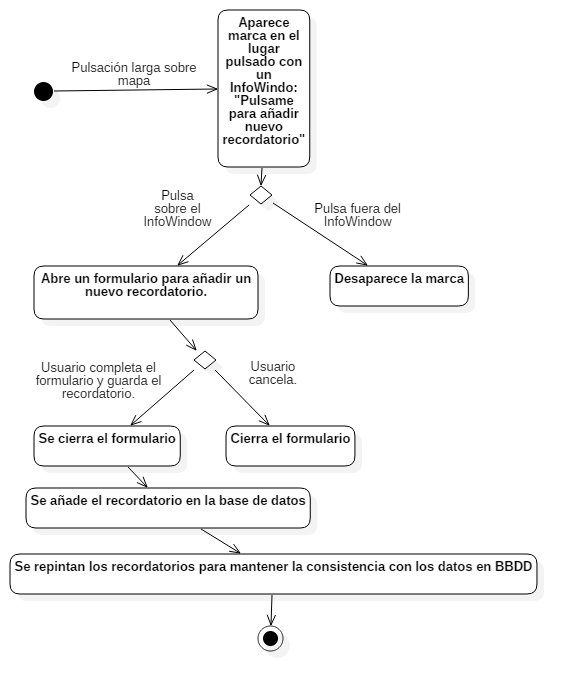
\includegraphics[width=0.8\textwidth]{Figures/ch2/ReminderMap/add_reminder_diagram}
    \caption{Diagrama de actividad que muestra la creación de un nuevo recordatorio.}
\end{figure}

Los elementos con los que el usuario interactuará durante el proceso (marca en el mapa, inforwindow, \ldots) son elementos que el propio framework pone a disposición del desarrollador, por lo que no tenemos que preocuparnos de implementarlos (diseñarlos, escribir el HTML, crear funciones que controlen la lógica, \ldots), lo cual supone un ahorro de tiempo considerable.

Modificaremos el código de nuestro \emph{MapComponent} de la siguiente manera:

\begin{lstlisting}[style=htmlcssjs,frame=tlrb,xleftmargin={0.2cm}]
  loadMap() {
    // RESTO DE LA FUNCIÓN

    this.map.on(GoogleMapsEvent.MAP_LONG_CLICK).subscribe((latLng) => {
      this.showAddNewReminderInfoWindow(latLng);
    });
  }

  showAddNewReminderInfoWindow(latLng: GoogleMapsLatLng) {
    let markerOptions: GoogleMapsMarkerOptions = {
      'position': latLng,
      // En las opciones de la marca, podemos configurar el infoWindow asociado a esta.
      'title': 'NUEVO RECORDATORIO'
      'snippet': "Click sobre mí si quieres añadir un nuevo recordatorio en esta localización.",
      'infoClick': (marker) => {
        // Se elimina la marca del mapa y se abre el formulario para añadir un nuevo recordatorio.
        marker.remove();
        this.showAddNewReminderPrompt(latLng);
      }
    };

    // Añadimos la marca al mapa, y cuando esté lista, hacemos que muestre en el infoWindow.
    this.map.addMarker(markerOptions).then((marker: GoogleMapsMarker) => {
      marker.showInfoWindow();
    });
  }

  showAddNewReminderPrompt (latLng: GoogleMapsLatLng) {
    // Deshabilitamos la interacción con el mapa
    this.map.setClickable( false )
    let prompt = this.alertCtrl.create({
      // Elegimos El mensaje que queremos que aparezca en nuestro formulario
      title: 'Nuevo recordatorio',
      message: "Se creará un nuevo recordatorio para la localización seleccionada.",
      // Configuramos los diferentes inputs que va a tener nuestro formulario indicando el texto que se mostrará y el nombre con el que será identificado este valor a la hora de devolver el los datos introducidos.
      inputs: [
        {
          name: 'name',
          placeholder: 'Nombre'
        },
        {
          name: 'description',
          placeholder: 'Descripción',
          type: 'text'
        },
      ],
      // También configuramos los botones que queremos que aparezcan, en este caso indicamos el texto del botón y la acción a realizar
      buttons: [
        {
          text: 'Cancelar',
          handler: data => { console.log('Cancel clicked');
          }
        },
        {
          text: 'Guardar',
          handler: data => {
            this.remindersProvider.reminders.addReminder(data['name'], data['description'], latLng);
          }
        }
      ]
    });
    // Hacemos que la iteración con el mapa se vuelva a habilitar cuando el formulario se cierre
    prompt.onDidDismiss(() => this.map.setClickable( true ));
    // Mostramos el formulario
    prompt.present();
  }
\end{lstlisting}

Se puede ver que se ha añadido al método \emph{loadMap()} una nueva instrucción para capturar el evento asociado a las pulsaciones largas sobre el mapa. Este evento lleva asociado las coordenadas sobre la que se ha pulsado. Cuando esto se produce, se ejecuta la función que hace que aparezca una marca sobre el mapa. Como comentaba antes, este elemento lo ofrece el propio framework, en este caso, a través del plugin de Google Maps. Para crearlo, se utiliza el método \emph{addMarker()} de nuestro mapa (que fue instanciado en el constructor), al cuál se le pasa un objeto de tipo \emph{GoogleMapsMarkerOptions} con la configuración de la marca y el InfoWindow asociado. Para ver más opciones, se puede consultar la documentación de este elemento en la página de Github \footnote{\url{https://github.com/mapsplugin/cordova\-plugin\-googlemaps/wiki/marker}}. El método \emph{addMarker()} devuelve una promesa, lo que nos permite ejecutar código en el momento en el que la marca esté lista. Vamos a aprovechar esta promesa para hacer que muestre el infoWindow asociado a la marca.

En caso de que el usuario pulse sobre el InfoWindow, se ejecutará el método \emph{showAddNewReminderPrompt()} que hará que aparezca un formulario con el cual añadir un nuevo recordatorio. Al igual que con las marcas, este formulario será implementado utilizando componentes que ofrece el Ionic. En este caso nos aprovecharemos del servicio de alertas, el cual no es más que un \emph{provider} que podemos inyectar desde el constructor y que permite la creación ventanas flotantes en nuestra aplicación. Para ello, solamente tenemos que llamar al método \emph{create()} del servicio de alertas pasandole la configuración que deseamos. En la documentación de Ionic podemos ver que parametros podemos configurar\footnote{\url{http://ionicframework.com/docs/v2/components/\#alert}}.

\warningbox{A la hora de mostrar el formulario, necesitamos deshabilitar la iteración con el mapa. ¿A que se debe esto?. Para comprenderlo, debemos saber que el mapa que se muestra no se renderiza con el vista web, si no que se trata de otra vista que se coloca por detrás. Es el propio plugin el que se encarga de hacer transparentes los elementos \emph{HTML} que contiene el mapa. Por esta razón, la propia alerta no puede gestionar por si misma la iteración con el mapa, y siendo por tanto tarea del desarrollador realizar esta gestión. Esto se aplica no solo para el formulario, también para cualquier otro elemento \emph{HTML} que se encuentre por encima del mapa y que se encuentren fuera del elemento que contiene el mapa\footnote{\url{https://github.com/mapsplugin/cordova-plugin-googlemaps/wiki/Map}}}

Ahora veamos los cambios a realizar para dibujar sobre el mapa los recordatorios que tenemos en la \gls{BBDD}. Recorreremos la lista de recordatorios que nos proporciona el \emph{ReminderProvider} e iremos creando marcas en el mapa para cada uno de ellos. En este caso, almacenaremos estas marcas en una colección en la que relacionaremos cada marca con el recordatorio correspondiente para poder usarlo más adelante, en una funcionalidad que implementaremos cuando veamos el componente \emph{ListComponent}. También dibujaremos un círculo cuyo centro será la marca y que representará el área de influencia del recordatorio seremos notificados. Este círculo se dibujara utilizando el método \emph{addCircle}\footnote{\url{https://github.com/mapsplugin/cordova-plugin-googlemaps/wiki/Circle}} del mapa.

\begin{lstlisting}[style=htmlcssjs,frame=tlrb,xleftmargin={0.2cm}]
  private markers : Map<Reminder, GoogleMapsMarker> = new Map<Reminder, GoogleMapsMarker>();

  // Esta función genera un color aleatorio.
  static getRandomColor () {
    return '#' + ('00000'+(Math.random()*(1<<24)|0).toString(16)).slice(-6);
  }

  loadMap() {
    // RESTO DE LA FUNCIÓN
    this.map.on(GoogleMapsEvent.MAP_READY).subscribe(() => {
        console.log('Map is ready!');
        this.drawReminderMarkers(this.remindersProvider.reminders.all());
        // Nos subscribimos al evento implementado en ReminderList para poder actualizar el mapa cuando se produzca una modificación en los datos.
        this.remindersProvider.reminders.onUpdate.subscribe(reminders => this.drawReminderMarkers(reminders))
    });
  }

  drawReminderMarkers(reminders: Array<Reminder>) {
    // Limpiamos el mapa de todo lo que tenga ya dibujado y reseteamos el registro de marcas.
    this.map.clear();
    this.markers.clear();

    for (let rem of reminders) {
      // Generamos el color de manera aleatoria, consiguiendo una mejor presentación.
      let color = MapPage.getRandomColor();

      let markerOptions: GoogleMapsMarkerOptions = {
        'icon': color,
        'position': rem.latLng,
        'title': rem.name,
        'snippet': rem.description,
        'markerClick': (marker: GoogleMapsMarker) => {
                          marker.showInfoWindow();
                        }
      };

      // Si la marca se ha añadido correcetamente, la guardamos y dibujamos el circulo a su alrededor.
      this.map.addMarker(markerOptions).then((marker: GoogleMapsMarker) => {
        this.markers.set(rem, marker);
        this.map.addCircle({
          'center': rem.latLng,
          'strokeColor' : color,
          'strokeWidth': 1,
          'radius': 100,
          'fillColor' : color
        });
      });
    }
  }
\end{lstlisting}

Estás marcas tendrán un infoWindow asociado, que a diferencia de la marca que se usa para añadir recordatorios, aparecerá cuando se pulse sobre la marca. En este infoWindow aparecerá información sobre el recordatorio.

También hemos modificado las acciones a realizar cuando el mapa este listo para que dibuje los recordatorios y para subscribirse al evento de refresco de datos que implementamos en la clase \emph{ReminderList}. Así, cada vez que se emita este evento, el mapa redibujara los recordatorios.

Con esto, podemos volver a probar la aplicación y comprobar como podemos añadir nuevos recordatorios y ver los ya registrados sobre el mapa, lo cual es recomendable antes de pasar a la siguiente funcionalidad.

\subsubsection{La lista}

Además de en el mapa, el usuario podrá ver los recordatorios en una lista, lo que le facilitará el ver los detalles de estos de un simple vistazo. Utilizaremos el componente de \textbf{ion-list} (que ya hemos utilizado para realizar el \nameref{sec:crono}) para crear esta lista. Además, cada uno de los items de esta lista serán del tipo \textbf{ion-item-sliding}\footnote{\url{http://ionicframework.com/docs/v2/components/\#sliding-list}}. Este tipo de componente permite añadir botones que se encuentran ``debajo'' de la opción y a los cuales podremos acceder deslizando el elemento en cuestión.

Veamos en primer lugar las modificaciones a realizar en el fichero \gls{HTML} de la página para añadir esta lista:

\begin{lstlisting}[style=htmlcssjs,frame=tlrb,xleftmargin={0.2cm}]
  <ion-content padding>
    <ion-list>
      <ion-item-sliding *ngFor="let reminder of remindersProvider.reminders.all()" >
        <ion-item>
          <h1> {{ reminder.name }} </h1>
          <p> {{ reminder.description }} </p>
        </ion-item>
        <ion-item-options side="right" >
          <button ion-button color="secondary" (click)="onClickMap(reminder)" >
            <ion-icon name="map" ></ion-icon>
            Mapa
          </button>
          <button ion-button color="danger" (click)="onClickRemove(reminder)" >
            <ion-icon name="trash" ></ion-icon>
            Eliminar
          </button>
        </ion-item-options>
      </ion-item-sliding>
    </ion-list>
  </ion-content>
\end{lstlisting}

El funcionamiento es simple, se recorre la lista de recordatorios y por cadad uno de ellos, se añade un item a la lista. Este item estará formado además de por el item propiamente dicho, en el que aparecen los datos del recordatorio, por dos botones que aparecerán cuando arrastremos el item. Uno de estos botones se usará para para eliminar el recordatorio, el otro, para abrir el mapa centrado en el recordatorio en cuestión.

En \emph{ListComponent}, tendremos que implementar los métodos a los que llaman los dos botones anteriormente nombrados.

\begin{lstlisting}[style=htmlcssjs,frame=tlrb,xleftmargin={0.2cm}]
  constructor(public navCtrl: NavController, public remindersProvider: ReminderProvider,
    public events: Events) {}

  onClickRemove(rem: any) {
    this.remindersProvider.reminders.removeReminder(rem);
  }

  onClickMap(rem: any) {
    this.events.publish('centerOnReminder:map', rem);
    this.navCtrl.parent.select(0);
  }
\end{lstlisting}

En método \emph{onClickRemove{}} no tiene más misterio que el de llamar al método \emph{removeReminder} de la clase \emph{ReminderList} pasando como parámetro el recordatorio a eliminar.

En cuanto al método \emph{onClickMap}, vemos como hacemos uso de dos \emph{providers} del sistema. El primero de ellos, \emph{Events}, nos permitirá emitir un evento al que, como veremos a continuación, nos deberemos subscribir desde \emph{MapComponent}, seleccionando el nombre del evento (\textbf{'centerOnReminder:map'}) y pudiendo pasar cualquier objeto al subscriptor, en este caso el recordatorio en cuestión. El cuando a \emph{NavController}\footnote{\url{http://ionicframework.com/docs/v2/api/components/tabs/Tabs/}}, se trata del controlador de la navegación a través del cual podremos acceder al componente \textbf{tabs} que contiene la página (valor de \emph{parent} dentro del \emph{NavController}), y cambiar de pestaña programáticamente. Ya que el mapa es la primera pestaña, la identificamos con el valor 0.

Por último, volvemos a \emph{MapController} para realizar la subscripción al evento \textbf{'centerOnReminder:map'} e implementar la función que centre el mapa sobre el marcador.

\begin{lstlisting}[style=htmlcssjs,frame=tlrb,xleftmargin={0.2cm}]
  constructor(public navCtrl: NavController, public platform: Platform, public remindersProvider: ReminderProvider, public alertCtrl: AlertController, public events: Events) {
    // RESTO DE LA FUNCIÓN
    events.subscribe('centerOnReminder:map', (rem) => this.centerOnReminder(rem));
  }
  centerOnReminder(rem: Reminder) {
    // El guardar la el recordatorio y la marca en un Map, nos permite realizar búsquedas utilizando el recordatorio.
    let marker = this.markers.get(rem);
    marker.getPosition().then((latLng) => this.map.setCenter(latLng));
    marker.showInfoWindow();
  }
\end{lstlisting}

\subsubsection{Las notificaciones}

Por último, debemos implementar la función principal para la que ha sido pensada esta aplicación, y es la de notificar al usuario cuando esté cerca de un recordatorio.

Para hacer esto, habrá que registrar un nuevo \emph{GeoFence}\footnote{\url{https://ionicframework.com/docs/v2/native/geofence/}} a la hora de crear un recordatorio. Este \emph{GeoFence} se activará cuando el dispositivo entre dentro del área de influencia de un recordatorio y se encargará de lanzar una notificación que aparecerá en la barra de notificaciones como las de cualquier otra aplicación. Este proceso se ejecuta aunque nuestra aplicación esté apagada, y podremos configurar el \emph{GeoFence} para que si el usuario pulsa sobre la notificación, se lance la aplicación. El código de creación y eliminación de estos \emph{GeoFence} formará parte de la clase \emph{Reminder}.

\begin{lstlisting}[style=htmlcssjs,frame=tlrb,xleftmargin={0.2cm}]
  createAssociatedGeoFence() {
  let fence = {
    id: this._id.toString(), // Utilizaremos el id del recordatorio también como id de la notificación para después poder eliminarla.
    latitude: this._lat,
    longitude: this._lng,
    radius: 100, // Radio en metros de la circunferencia que define el área de influencia del recordatorio.
    transitionType: 1, // Enter transition
    // Configuración de la notificación. En ella aparecerá la información sobre el recordatorio.
    notification: {
        id:             1,
        title:          this._name,
        text:           this._description,
        openAppOnClick: true
    }
  }

  Geofence.addOrUpdate(fence).then(
   () => console.log('Geofence added'),
   (err) => console.log(err)
 );
}

removeAssociatedGeoFence() {
  Geofence.remove(this._id.toString()).then(
   () => console.log('Geofence removed'),
   (err) => console.log('Geofence failed to remove')
 );
}
\end{lstlisting}

Debemos asegurarnos de llamar a estás funciones cada vez que se inserte o se elimine un recordatorio en la \gls{BBDD}. Estando seguros de que la operación se ha realizado con éxito para intentar mantener la coherencia entre los \emph{geofences} registrados y los recordatorios guardados.
